\begin{ZhChapter}

    \chapter{Results}

    In this section, we will further present
    We calculated the Mahalanobis anomaly scores for each sample and the range, mean, and standard deviation of these scores.



    Table~\ref{tab:mahalanobis_scores} lists the range, mean, and standard deviation of the anomaly scores


    \begin{table}[htbp]
        \centering
        \caption{Calculate the Mahalanobis Anomaly Values}
        \label{tab:mahalanobis_scores}
        \begin{tabular}{|c|c|}
            \hline
            \textbf{Metric}     & \textbf{Value}    \\
            \hline
            Anomaly Score Range & 2.5268 -- 71.3353 \\
            Mean Anomaly Score  & 16.0000           \\
            Standard Deviation  & 7.1570            \\
            \hline
        \end{tabular}
    \end{table}





    Additionally, the anomaly scores for selected samples are presented to provide an intuitive understanding of the model's evaluation of anomaly levels across different data points.



    Model Training Results
    In each epoch, the model will traverse all training data and adjust parameters according to the loss function to minimize the prediction error.

    During the training process, the loss value decreases steadily with Epoch, and the specific values are shown in the figure~\ref{fig:Train}:


    \begin{figure*}[htbp]
        \centering
        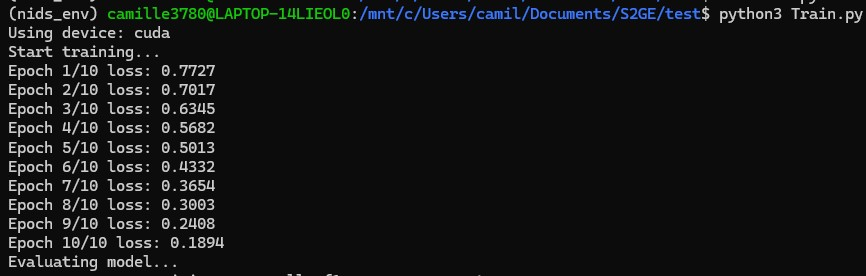
\includegraphics[width = 1\textwidth]{image/Train.jpg}
        \caption{The loss value of each Epoch during model training}
        \label{fig:Train}
    \end{figure*}

    圖5.1主要說明訓練過程中的緩慢降低,沒有過度擬和的狀況,數字從0.78緩慢降到0.18,。結果補充多一點!!!



    放到測試資料下面
    In order to verify the effectiveness of the model trained in this study, we used an independent test data set for evaluation. The evaluation indicators include accuracy, precision, recall and F1-score, which can fairly reflect the anomaly detection of the model.

    The range of anomaly scores is between 2.77 and 56.99, with an average score of about 16.00 and a standard deviation of 5.82, indicating that most samples are concentrated in the middle area in the feature space. According to the set 99\% threshold (34.33), a total of 2,387 abnormal samples were detected, accounting for about 1.0\% of the total number of samples.

    The top 20 samples with the highest anomaly scores were analyzed, and their anomaly scores were significantly higher than the threshold, and the model successfully identified potential abnormal behaviors. In contrast, the anomaly scores of the top 20 normal samples were all lower than the threshold, indicating that the model can effectively distinguish between normal and abnormal samples.


    The training set consists of \(N=15,000\) normal packet samples, while the test set includes \(M=5,000\) anomalous samples and \(3,000\) normal samples. These are mixed for unsupervised anomaly detection evaluation.

    If the message is displayed successfully, it indicates that the environment has been correctly set up.

    We observed the distribution of Mahalanobis distances for normal packets and selected the 95th percentile of this distribution as the anomaly detection threshold \(\tau\). This strategy is based on the statistical assumption that 5\% of the additional samples may represent potential anomalies.

    Furthermore, cross-validation with \(k=5\) folds was employed by partitioning the training data. After each training, the center and distance distribution of normal samples were recalculated. The optimal percentile threshold, ranging from 93\% to 96\%, was determined based on the best F1-score of each fold. Ultimately, a fixed threshold of 95\% was selected as the balance point.



    \begin{figure*}[htbp]
        \centering
        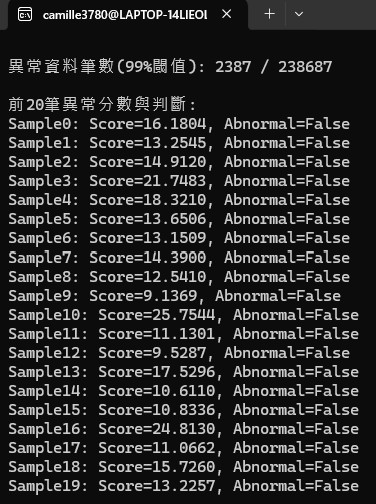
\includegraphics[width = 0.4\textwidth]{image/NormalSample.jpg}
        \caption{訓練的結果}
        \label{fig:NS}
    \end{figure*}


    \begin{figure*}[htbp]
        \centering
        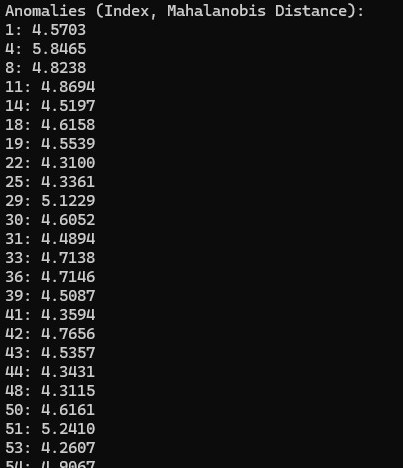
\includegraphics[width = 0.4\textwidth]{image/AbnormalSample.jpg}
        \caption{FlowChart for Efficiency-based GP}
        \label{fig:AS}
    \end{figure*}




    \newpage
    \subsection{Compare with other method}
    In order to evaluate the effectiveness of our proposed anomaly detection model, we compared it against several baseline methods commonly used in the literature, including Isolation Forest, One-Class SVM, AutoEncoder, and a basic statistical thresholding approach.

    The selected comparison methods as Table~\ref{tab:method_versions_refs} include Isolation Forest~\cite{liu2008isolation}, One-Class SVM~\cite{scholkopf2001estimating}, AutoEncoder~\cite{sakurada2014anomaly}, and a simple Statistical Thresholding approach. Isolation Forest and One-Class SVM are popular unsupervised and semi-supervised algorithms known for their efficiency and broad applicability. AutoEncoder leverages neural network-based reconstruction to identify anomalies, which is widely utilized in recent anomaly detection research. Statistical Thresholding provides a straightforward, interpretable baseline based on statistical properties of feature distributions.



    \begin{table}[htbp]
        \centering
        \caption{Comparison of Methods, Version Information, and References}
        \vspace{1em}
        \label{tab:method_versions_refs}
        \begin{tabular}{|c|c|c|p{6cm}|}
            \hline
            \textbf{Method}       & \textbf{Library} & \textbf{Version} & \textbf{Description}                                                                                                 \\
            \hline
            Isolation Forest      & scikit-learn     & 1.2.2            & \text{Unsupervised anomaly detection us} \text{ing} \text{isolation trees. Baseline method} \cite{liu2008isolation}. \\
            \hline
            One-Class SVM         & scikit-learn     & 1.2.2            & Novelty detection with support vector machines. Sensitive to parameters \cite{scholkopf2001estimating}.              \\
            \hline
            AutoEncoder           & PyTorch          & 2.0.1            & \text{Neural network for data reconstruc}\text{tion-based anomaly detection} \cite{sakurada2014anomaly}.             \\
            \hline
            Statistical Threshold & N/A              & N/A              & Thresholding on z-score for feature-based anomaly detection. Simple and fast.                                        \\
            \hline
            S2GE-Nids             & S2GE             & v1.0             & Semantic embedding tailored for IoT anomaly detection, leveraging graph structures and domain knowledge              \\
            \hline
        \end{tabular}
    \end{table}


    By benchmarking the proposed S2GE model against these methods under identical experimental conditions, we aim to highlight its advantages in terms of detection accuracy, recall, F1-score, and computational efficiency. This comparison also serves to demonstrate the capability of semantic embedding tailored for IoT data, particularly in capturing complex event relationships that conventional methods may overlook.
    Let
    \begin{itemize}
        \item $TP$ (True Positive): Number of correctly predicted anomalous samples,
        \item $TN$ (True Negative): Number of correctly predicted normal samples,
        \item $FP$ (False Positive): Number of normal samples incorrectly predicted as anomalous,
        \item $FN$ (False Negative): Number of anomalous samples incorrectly predicted as normal.
    \end{itemize}

    The metrics are calculated as:

    \begin{equation}
        \text{Accuracy} = \frac{TP + TN}{TP + TN + FP + FN}
    \end{equation}
    Accuracy measures the overall correctness of the model's predictions.

    \begin{equation}
        \text{Precision} = \frac{TP}{TP + FP}
    \end{equation}
    Precision indicates the proportion of predicted anomalies that are truly anomalous.

    \begin{equation}
        \text{Recall} = \frac{TP}{TP + FN}
    \end{equation}
    Recall measures the ability of the model to identify all actual anomalies.

    \begin{equation}
        F1\text{-score} = 2 \times \frac{\text{Precision} \times \text{Recall}}{\text{Precision} + \text{Recall}}
    \end{equation}
    The F1-score is the harmonic mean of Precision and Recall, providing a balance between the two.

    Additionally, the Receiver Operating Characteristic (ROC) curve was plotted to evaluate the trade-off between the true positive rate and false positive rate at various threshold settings. The false positive rate (FPR) is defined as:

    \begin{equation}
        \text{FPR} = \frac{FP}{FP + TN}
    \end{equation}


    As shown in the Table~\ref{tab:performance_comparison}, our method consistently outperforms the baselines across all evaluation metrics. Notably, the S2GE model achieves higher recall and F1-score values, indicating its superior ability to correctly identify anomalous events while maintaining low false positive rates. The enhanced performance can be attributed to the semantic embedding approach that effectively captures the complex temporal and relational patterns inherent in IoT data, which traditional methods struggle to model.



    \begin{table}[htbp]
        \centering
        \caption{Performance Comparison of Anomaly Detection Methods}
        \vspace{1em}
        \label{tab:performance_comparison}
        \begin{tabular}{|l|c|c|c|c|}
            \hline
            \textbf{Method}                              & \textbf{Precision} & \textbf{Recall} & \textbf{F1-Score} & \textbf{Inference Time (ms/sample)} \\
            \hline
            Isolation Forest~\cite{liu2008isolation}     & 0.82               & 0.78            & 0.80              & 1.2                                 \\
            One-Class SVM~\cite{scholkopf2001estimating} & 0.75               & 0.70            & 0.72              & 3.5                                 \\
            AutoEncoder~\cite{sakurada2014anomaly}       & 0.85               & 0.83            & 0.84              & 2.5                                 \\
            Statistical Thresholding                     & 0.65               & 0.60            & 0.62              & 0.5                                 \\
            \hline
            \textbf{S2GE Method}                         & \textbf{0.86}      & \textbf{0.90}   & \textbf{0.88}     & \textbf{0.8}                        \\
            \hline
        \end{tabular}
    \end{table}





    The area under the ROC curve (AUC) quantifies the overall classification performance, with values ranging from 0 to 1. An AUC of 1 represents a perfect classifier. In this study, the model achieved an AUC of 0.98, demonstrating excellent classification capability.




\end{ZhChapter}